\documentclass[12pt, letterpaper]{report}
\usepackage[utf8]{inputenc}
\usepackage[T1]{fontenc}
\usepackage[english,polish]{babel}
\usepackage{fancyhdr}
\usepackage{hyperref}
\usepackage{wrapfig}
\usepackage{subcaption}
\usepackage{graphicx}
\usepackage{multicol}
\usepackage{blindtext}
\usepackage{amsmath}
\usepackage{float}
\usepackage{listings}
\usepackage{xcolor}
\usepackage[margin=1.5cm]{geometry}

\graphicspath{ {images/} {images/collisions24x10_2x2} }

\definecolor{codegreen}{rgb}{0,0.6,0}
\definecolor{codegray}{rgb}{0.5,0.5,0.5}
\definecolor{codepurple}{rgb}{0.58,0,0.82}
\definecolor{backcolour}{rgb}{0.95,0.95,0.92}

\lstdefinestyle{codelistingstyle}{
    backgroundcolor=\color{backcolour},   
    commentstyle=\color{codegreen},
    keywordstyle=\color{magenta},
    numberstyle=\tiny\color{codegray},
    stringstyle=\color{codepurple},
    basicstyle=\ttfamily\footnotesize,
    breakatwhitespace=false,         
    breaklines=true,                 
    captionpos=b,                    
    keepspaces=true,                 
    numbers=left,                    
    numbersep=5pt,                  
    showspaces=false,                
    showstringspaces=false,
    showtabs=false,                  
    tabsize=2
}

\lstset{style=codelistingstyle}

\title{
    Raport z postępów pracy \\
    \large Modelowanie elastycznych i nieelastycznych
    zderzeń obiektów\\
    metodą dynamiki molekularnej na potrzeby animacji
    komputerowych
}
\author{
    Kamil Pasterczyk \\
    \small Promotor: dr hab. inż. Tomasz Chwiej
}

\begin{document}

\maketitle
\tableofcontents

\chapter{Wstęp}
    \section{Cele projektu}
    Jedną z popularnych metod wykorzystywanych w modelowaniu zderzeń obiektów w mikro- i makroskali jest 
    metoda dynamiki molekularnej. Mimo iż w pierwotnej postaci stosowana była do opisu własności gazów i 
    cieczy, to dzięki swej wszechstronności pozwala modelować obiekty makroskopowe zachowujących kształt 
    przy braku sił zewnętrznych oraz modelować ich rozrywanie w trakcie zderzeń z innymi obiektami. W pracy 
    należy zaadoptować odpowiednio sparametryzowany model dynamiki molekularnej i na jego podstawie opracować 
    algorytmy numeryczne do symulacji zderzeń obiektów z możliwością penetracji lub rozrywania jednego z nich. 
    Algorytmy powinny być zaimplementowany na tyle wydajne aby możliwa była wizualizacja zderzeń w czasie 
    rzeczywistym jako animacje komputerowe.

    \section{Model oddziaływań}
    Potencjał Lennarda-Jonesa został wykorzystany do symulacji przyciągania/odpychania 
    węzłów w jednym obiekcie, symulacji kolizji węzłów ze ścianami oraz symulacji
    kolizji węzłów z węzłami należącymi do innych obiektów. 
    Potencjał ten opisany jest za pomocą poniższego równania:
    \begin{equation}
        E_{LJ} = V_0 \left[ \left( \frac{\sigma}{l} \right)^{12} - \left( \frac{\sigma}{l} \right)^{6} \right]
    \end{equation}
    \begin{equation}
        \sigma = \frac{d_0}{\sqrt[6]{2}}
    \end{equation}
    Gdzie $l$ to odległość między dwiema oddziałującymi cząstkami, $V_0$ to współczynnik określający wielkość potencjału 
    a $\sigma$ to odległość, przy której energia potencjalna odziaływania pomiedzy cząsteczkami wynosi zero. 
    Potencjał Lennarda-Jonesa ma swoje minimum w odległości $d_0 = \sqrt[6]{2} \sigma$. \\ \\
    Siła zdefiniowana jest jako pochodna energii:
    \begin{equation}
        F_{LJ} = 
        \frac{d}{dl} E_{LJ} = 
        \frac{d}{dl} V_0 \left[ \left( \frac{\sigma}{l} \right)^{12} - \left( \frac{\sigma}{l} \right)^{6} \right]
    \end{equation}
    \begin{align*}
        F_{LJ} &= \frac{d}{dl} V_0 \left[ \sigma^{12}l^{-12} - \sigma^{6}l^{-6} \right] =\\
        &= V_0 \left[ \sigma^{12}(-12)l^{-13} - \sigma^{6}(-6)l^{-7} \right] =\\
        &= V_0 \left[ 6\sigma^{6}l^{-7} - 12\sigma^{12}l^{-13} \right] =\\
        &= V_0 \left[ 6 \left(\frac{d_0}{\sqrt[6]{2}}\right)^{6} l^{-7} - 12 \left(\frac{d_0}{\sqrt[6]{2}}\right)^{12} l^{-13} \right] =\\
        &= 3 V_0 \left[ 2 \left(\frac{d_0}{\sqrt[6]{2}}\right)^{6} l^{-7} - 4 \left(\frac{d_0}{\sqrt[6]{2}}\right)^{12} l^{-13} \right] =\\
        &= 3 V_0 \left[ (d_{0})^{6} l^{-7} - (d_{0})^{12} l^{-13} \right] =\\
        &= 3 \frac{V_0}{d_0} \left[ (d_{0})^{7} l^{-7} - (d_{0})^{13} l^{-13} \right] =\\
        &= 3\frac{V_0}{d_0} \left[ \left(\frac{d_0}{l}\right)^{7} - \left(\frac{d_0}{l}\right)^{13} \right]
    \end{align*}
    W ten sposób otrzymaliśmy wzór opisujący siłę wynikającą z potencjału Lennarda-Jonesa:
    \begin{equation}
        F_{LJ} = 3\frac{V_0}{d_0} \left[ \left(\frac{d_0}{l}\right)^{7} - \left(\frac{d_0}{l}\right)^{13} \right]
    \end{equation}

    \section{Wizualizacja temperatury}
    \subsection{Temperatura z teorii gazów}
    Punktem wyjścia moe być zasada ekwipartycji energii: średnia energia kintetyczna na jeden stopień swobody jest równa 
    $\frac{k_{B}T}{2}$ gdzie $k_{B}$ to stała Boltzmana a $T$ to temperatura.

    \begin{equation}
        \left< E_{k} \right> = s \frac{k_{B}T}{2}
    \end{equation}

    W naszym przypadku liczba stopni swobody $s = 2$ (ruch translacyjny w dwóch osiach $x$ i $y$).

    \begin{align*}
        \left< E_{k} \right> = \left< \frac{m v^{2}}{2} \right> = \frac{m}{2} \left< v^{2} \right> = T \frac{k_{B}}{2}
    \end{align*}

    \begin{equation}
        T = \frac{m}{k_{B}} \left< v^{2} \right>
    \end{equation}

    Wzór wzięty z teorii kinetyczno-molekularnej gazów.

    \subsection{Weryfikacja poprawności wzoru}
    Rozważmy przypadek gdy obiekt porusza się w przestrzeni jako całość: swobodny spadek w polu grawitacyjnym.
    Węzły nie drgają i przepieszczają się z tą samą prędkością 
    $\vec{V_k} = \vec{V_0} + \vec{g}t$ dla $t > 0  \Rightarrow  |\vec{V_k}|^2  \Rightarrow  T > 0$ a 
    przecież swobodny spadek nie rozgrzewa ciał. 
    Wniosek: ten wzór jest nieodpowiedni dla naszego modelu, należy go zmodyfikować.
    
    \subsection{Modyfikacja wzoru}
    Należy przeskalować prędkość, to znaczy odjąć średnią prędkość z jaką porusa się obiekt jako całość, wówczas nie będzie
    to prowadziło dodadkowego wzrosu temperatury. Def: $\left< v^{2} \right>  =  \frac{1}{T} \int_{0}^{T} v^2(t) dt$
    uśredniony po krótkich odcinkach czasu. Estymator $\left< v^{2} \right>$ to średnia arytmetyczna: 
    $t = t_i = i \cdot \Delta t$ dla $i = 0, 1, ..., n-1$.

    \begin{equation}
        \left< v^{2} \right>  \approx  \overline{v^2} = \frac{1}{n \cdot \Delta t} \sum_{i = 0}^{n} {v_i}^2 \Delta t
        = \frac{1}{n} \sum_{i = 0}^n {v_i}^2
    \end{equation}

    Modyfikujemy wzór odejmująć wartość średnią:
    \begin{align*}
        \left< \left( v - \left< v \right> \right)^2 \right>  &=  
        \frac{1}{T} \int_{0}^{T} \left( v(t) - \left< v \right> \right)^2 dt  \\
        &= \frac{1}{T} \int_{0}^{T} \left( v^2(t) - 2v \left< v \right> + \left< v \right>^2 \right) dt  \\
        &= \frac{1}{T} \int_{0}^{T} v^2 \, dt - 2 \left< v \right> \frac{1}{T} \int_{0}^{T} v \, dt + \left< v \right>^2 
        + \left< v \right>^2 \frac{1}{T} \int_{0}^{T} dt \\
        &= \left< v^2 \right> - 2 \left< v \right> \cdot \left< v \right> + \left< v \right>^2 \\
        &= \left< v^2 \right> - \left< v \right>^2
    \end{align*}

    Uzyskany wynik to wariancja prędkości:
    \begin{equation}
        {\delta_v}^2  =  \left< \left( v - \left< v \right> \right)^2 \right>  =  \left< v^2 \right> - \left< v \right>^2
    \end{equation}

    Estymator wariancji:
    \begin{equation}
        {\delta_v}^2  \approx  \frac{1}{n} \sum_{i = 0}^{n - 1} {v_i}^2 - \left( \frac{1}{n} \sum_{i = 0}^{n - 1} {v_i} \right)^2
    \end{equation}

    \subsection{Weryfikacja zmodyfikowanego wzoru}
    Ponownie rozparzymy spadek swobodny dla jednego wymiaru: $v_k = v_0 + gt$ gdzie $v_0 = 0 = v_k = gt$

    \begin{align*}
        {\delta_v}^2  &=
        \left< v^2 \right> - \left< v \right>^2 \\ 
        &=  \frac{1}{T} \int_{0}^{T} g^2 t^2 \, dt  -  \left( \frac{1}{T} \int_{0}^{T} g \cdot t \, dt \right)^2  \\
        &=  g^2 \frac{1}{T} \frac{T^3}{3}  -  \left( g \frac{1}{T} \frac{T^2}{2} \right)^2  = \frac{g^2 T^2}{3}  -  \frac{g^2 T^2}{4} \\
        &=  \frac{g^2 T^2}{12}
    \end{align*}

    \begin{equation}
        {\delta_v}^2  =  \frac{g^2 T^2}{12}
    \end{equation}

    Temperatura wciąż wzrasta. Jeżeli jednak $a >> g$ to wpływ jest niewielki a dla $T << 1$ oraz $a >> g$ 
    np. $a = 5 \cdot g \Rightarrow {\delta_{v_a}}^2 = 25 \cdot {\delta_{v_g}}^2$

    \lstinputlisting[language=C]{code/temperature.c}

    \subsection{Temperatura z twierdzenia o wiriale}
    Prędkości węzłów zmieniają się w czasie, więc będzie też zmieniać się średnia energia kinetyczna układu.

    \begin{equation}
        \left< E_{kinetyczna} \right>  =  \left< \sum_{k = 1}^{N_p} \frac{m_k}{2} {v_k}^2 \right>
        = \sum_{k = 1}^{N_p} \frac{m_k}{2} \left< {v_k}^2 \right>
    \end{equation}

    Twierdzenie o wirale mówi że energia kinetyczna zamijnia się wskutek oddiaływań wewnętcznych i można go 
    liczyć ze wzoru:

    \begin{equation}
        \left< E_{kinetyczna} \right>  = 
         - \frac{1}{2} \sum_{k = 1}^{N_p} \left< \vec{F_k} \cdot \vec{r_k} \right>
    \end{equation}

    \begin{equation}
        \vec{F_k} = \sum_{j = 1}^{M} \vec{{F_k}_j}
    \end{equation}
    Gdzie $M$ to liczba sąsiadów a $\vec{{F_k}_j}$ to siła oddziaływania z sąsiadem $j$-tym.

    \begin{equation}
        \left< E_{kinetyczna} \right> = 
        \sum_{k = 1}^{N_p} -\frac{1}{2} \left< \vec{F_k} \cdot \vec{r_k} \right> =
        \sum_{k = 1}^{N_p} \left< E_{kinetyczna} , k \right>
    \end{equation}
    $\left< E_{kinetyczna} , k \right>$ to suma średnich energii kinetycznych węzłów. Dla każdego węzła $k$ możemy policzyć:

    \begin{equation}
        \left< E_{kinetyczna} , k \right> = 
        -\frac{1}{2} \frac{1}{\tau} \int_{0}^{\tau} \vec{F_k}(t) \cdot \vec{r_k}(t) \, dt
    \end{equation}
    Gdzie $\tau = \Delta t \cdot n$.

    \begin{equation}
        \left< E_{kinetyczna} , k \right> = 
        -\frac{1}{2} \frac{1}{n} \sum_{j = 0}^{n} \left[  F_{kx}(t_j) \cdot x_n(t_j) + F_{ky}(t_j) \cdot y_k(t_j) \right]
    \end{equation}
    Elementy sumy zapisywane są tak samo jak poprzednio w tablicy. Przyjmujemy $n > 100$ lub więcej. 

    \begin{equation}
        \left< E_{kinetyczna, k} \right> = k_B T_k \Rightarrow T_k = \frac{\left< E_{kinetyczna, k} \right>}{k_B}
    \end{equation}
    Gdzie $k_B$ tostała Boltzmanna.

    \begin{enumerate}
        \item Jeśli $\vec{F_n} = 0 \Rightarrow T_k = 0$ czyli temperatura taka jak otoczenie.
        \item Jeśli $\left< E_{kinetyczna, k} \right> < 0 \Rightarrow T_k < 0$ oznacza że lokalna temperatura stało się mniejsze niż w otoczeniu obiektu.
    \end{enumerate}

    \section{Wizualizacja ciśnienia}
    Węzeł otaczamy w komorze o boku $\Delta$. Zgodnie z definicją ciśnienie na ściankach można opisać wzorem:
    \begin{equation}
        P_x (x \pm \frac{\Delta}{2}) = \frac{F_x (x \pm \frac{\Delta}{2})}{\Delta}
    \end{equation}
    Siła:
    \begin{equation}
        F_x (x + \frac{\Delta}{2}) = F_x (x) + \frac{\partial F_x}{\partial x} 
        \left| _{x + \frac{x}{2}}  \frac{x}{2} + \frac{\partial^2 F_x}{\partial x^2 }  \right| \frac{\Delta^2}{4} + O(\Delta^3)
    \end{equation}
    \begin{equation}
        F_x (x - \frac{\Delta}{2}) = F_x (x) - \frac{\partial F_x}{\partial x} 
        \left| _{x - \frac{x}{2}}  \frac{x}{2} + \frac{\partial^2 F_x}{\partial x^2 }  \right| \frac{\Delta^2}{4} + O(\Delta^3)
    \end{equation} 
    \begin{equation}
        \Delta F_x = 
        F_x (x - \frac{\Delta}{2}) - F_x (x - \frac{\Delta}{2}) = 
        \frac{\Delta}{2} \left[ \frac{\Delta F_x}{\partial x} |_{x + \frac{\Delta}{2}}  -
          \frac{\Delta F_x}{\partial x}|_{x - \frac{\Delta}{2}} \right] + O(\Delta^2)
    \end{equation}
    Dzielimy równanie przez $\Delta$
    \begin{equation}
        p_x = \frac{\Delta F_x}{\Delta} = \frac{1}{2} 
        \left[ \frac{\partial F_x}{\partial x} |_{x + \frac{\Delta}{2}} - \frac{\partial F_x}{\partial x} |_{x - \frac{\Delta}{2}} \right] + O(\Delta)
    \end{equation}
    Podobnie liczymy dla kierunku $y$
    \begin{equation}
        p_y = \frac{\Delta F_y}{\Delta} = \frac{1}{2} 
        \left[ \frac{\partial F_y}{\partial y} |_{y + \frac{\Delta}{2}} - \frac{\partial F_y}{\partial y} |_{y - \frac{\Delta}{2}} \right] + O(\Delta)
    \end{equation}
    A następnie uśredniamy:
    \begin{equation}
        p_{srednie} = \frac{1}{2} \left( -p_x - p_y \right)
    \end{equation}
    Dodajemy minus ponieważ siła jest skierowana do środka komory a ciśnienie powinno być większe od zera.
    \begin{enumerate}
        \item $\Delta$ powinno być małe np. $\Delta = \frac{\delta_{LJ}}{20}$ gdzie $\delta_{LJ}$ to parametr potencjału Lennarda-Jonesa
        \item dla położenia $k$-tego węzła $\vec{r_k}$ trzeba policzyć 4 pochodną siły.
        \item pochodne eliminuje wpływ pola grawitacjnego, poniewać jest to wartość stała.
    \end{enumerate}

    \subsection{Testy poprawność wzoru}
    \begin{enumerate}
        \item Przypadek statyczny z jednym obiektem: Obiekt stojący na podłożu w polu grawitacyjnym.
        Większy nacisk będzie znajdować się przy podstawie obiektów.
        
        \item Przypadek dynamiczny: Uderzenie kulki w obiekt prostokątny. Największe ciśnienie 
        znajdzie się w miejscu zderzenia dwóch obiektów.

        \item Przypadek statyczny z dwoma obiektami: Dwa obiekty położone na sobie bez pola grawitacyjnego.
        Ciśnienie w środku powinno być jednorodne i takie sam jak u góry obiektu. Brzegi powinny się deformować.
    \end{enumerate}

\chapter{Testy}
    \section{Test poprawność działania algorytmów}
    \subsection{Opis testu}
    
    \begin{wrapfigure}{r}{0.45\textwidth}
        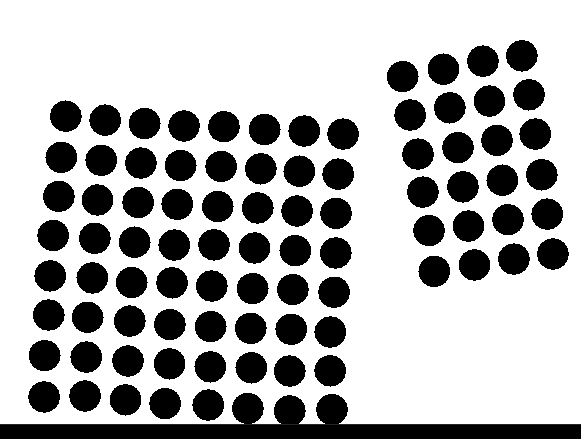
\includegraphics[width=0.9\linewidth]{objects_raw} 
        \caption{Widok aplikacji w fazie testów z widocznymi dwoma obiektami $8 \times 8$ oraz $6 \times 4$}
    \end{wrapfigure}
    Jeżeli wszystkie algorytmy symulujące odziaływania fizyczne zostały zimplementowane poprawnie 
    to w przypadku gdy nie występują żadne siły oporu energia całkowita układu powinna 
    być stała przez cały czas trwania symulacji. Aby uzyskać poprawny obraz sytuacji należy 
    uwzględnić wszystkie rodzaje energii w układzie: 
    \begin{enumerate}
        \item Energia potencjalna grawitacji
        \item Energia kinetyczna
        \item Energia potencjalna węwnątrz obiektu
        \item Energia potencjalna odpychająca pomiędzy obiektami a podłożem
        \item Energia potencjalna odpychająca pomiędzy dwoma obiektami
    \end{enumerate}
    Do testu zachowania energii wykorzystane są 
    dwa obiekty o rozmiarach odpowiednio $8 \times 8$ i $6 \times 4$ oraz statyczne podłoże. Obiekty
    znajdują się w polu grawitacyjnym, nie ma żadnych sił oporu/tarcia.

    \subsubsection{Parametry symulacji}
    \begin{align*}
        g &= 9.81 [\frac{m}{s^2}] \\
        dt &= 10^{-5} [s] \\
        t_{max} &= 8 [s]
    \end{align*}
    \pagebreak
    \subsection{Wyniki}
    \begin{figure}[h]
        \centering
        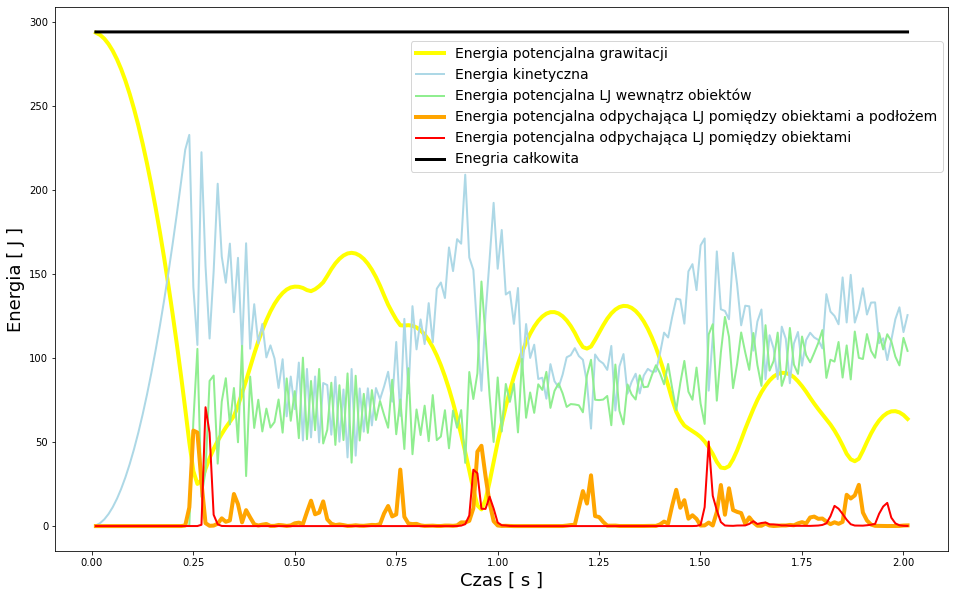
\includegraphics[width=13cm]{energy_test_0to2s}
        \caption{Zmiana enegii w czasie dla układu w ciągu pierwszych 1.2 sekund}
    \end{figure}

    Przy zderzeniach pomiędzy obiektami oraz pomiędzy obiektem i podłożem energia potencjalna
    odpychająca Lennarda-Jonesa oznaczona kolejno kolorami pomarańczowym i czerwonym
    wyraźnie wzrasta.
    \begin{figure}[h]
        \centering
        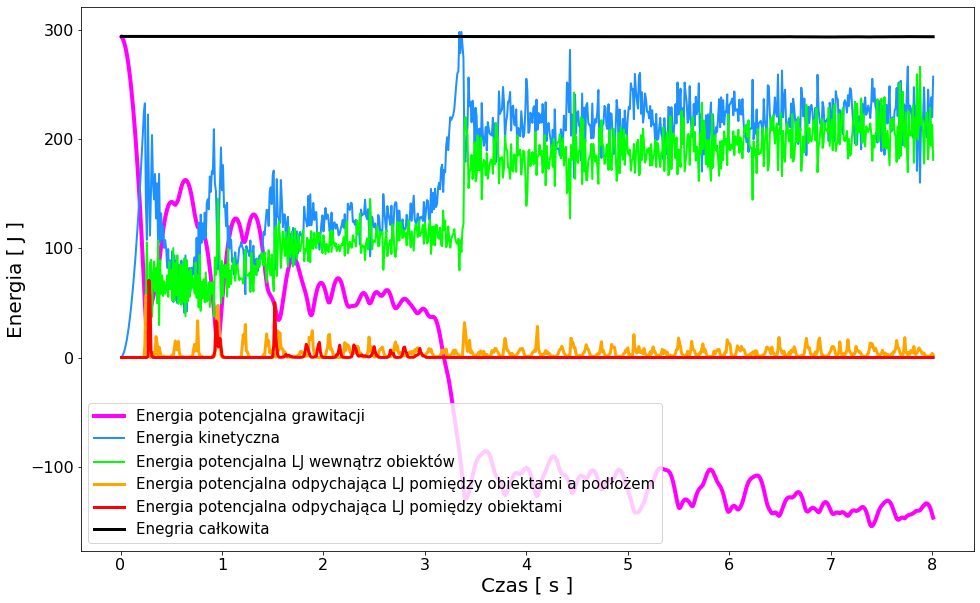
\includegraphics[width=13cm]{energy_test_0to8s}
        \caption{Zmiana enegii w czasie dla układu w ciągu pierwszych 8 sekund}
    \end{figure}
    
    Po upłynięciu kilku sekund obiekty zostają przy podłożu, energia będąca początkowo energią
    potencjalną grawitacji została w większości zamieniona na energię kinetyczną oraz energię
    wewnętrzną. Obiekty nie odbijają się one już między sobą.
    Zmiana energii całkowitej w czasie działania całej symulacji była mniejsza niż $1\%$. Na tej
    podstawie można uznać, że algorytmy zostały zaimplementowane poprawnie.


    \section{Test wydajności dla dwóch algorytmów obsługi zderzeń między obiektami}
    \subsection{Opis algorytmów}
    Naszym celem jest obliczanie siły poędzy odpowiednimi węzłami w taki sposób aby 
    obiekty przy zderzeniu odpychały się od siebie.
    
    \begin{figure}[h]

        \begin{subfigure}{0.5\textwidth}
        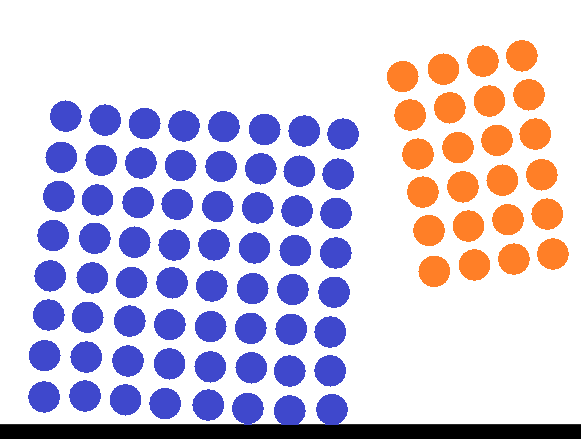
\includegraphics[width=0.9\linewidth, height=6cm]{objects_unoptimized} 
        \caption{Metoda "każdy z każdym"}
        \end{subfigure}
        \begin{subfigure}{0.5\textwidth}
        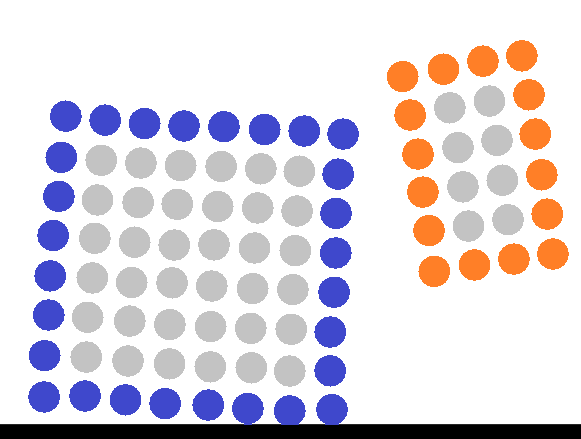
\includegraphics[width=0.9\linewidth, height=6cm]{objects_optimized}
        \caption{Metoda węzłów granicznych}
        \end{subfigure}
        
        \caption{Reprezentacja dwóch metod obsługi zderzeń}
    \end{figure}

    Dla metody (a) oddziaływanie liczone jest pomiędzy każdym węzłem o kolorze niebieskim z każdym węzłem o
    kolorze pomarańczowym. Metoda o złożoności $O(n^2)$ gdzie $n$ to liczba węzłów.
    Jest to metoda bardzo wolna, lecz dająca poprawne rezultaty w każdym symulowanym przypadku.\\

    Dla metody (b) oddziaływanie ponownie liczone jest pomiędzy każdym węzłem o kolorze niebieskim z każdym
    węzłem o kolorze pomarańczowym, tym razem jednak oznaczone są jedynie węzły brzegowe.
    Metoda ta jest szczególnie efektywna dla obiektów kwadratowych o boku $n$, gdzie z $n^2$
    rozpatrywanych węzłów ta liczba jest zmniejszona do zaledwie $4(n-1)$ węzłów.
    Należy zwrócić uwagę, że metoda ta nie będzie poprawnie odwzorowywać oddziaływań dla
    obiektów zagnieżdżonych w sobie. Przykładowa sytuacja, w której algorytm nie zadziała poprawnie
    to symulacja penetracji obiektu przy kuli/naboju.

    \subsection{Opis testu}
    Rozpatrujemy scenariusz z dwoma obiektami, sprawdzamy liczbę iteracji symulacji na sekundę stopniowo
    zwiększając liczbę węzłów w obydwóch obiektach. Test został wykonany na pojedynczym rdzeniu procesora AMD Ryzen 5 5600X, 
    ilość węzłów w bokach obiektów ustawiana jest kolejno na: 3, 5, 9, 10, 15, 21, 25, 30, 35, 40, 45, 50, 55, 60.
    
    \newpage
    \subsection{Wyniki}
    Wyniki z przeprowadzonego testu prezentują się następująco:
    \begin{figure}[H]
        \centering
        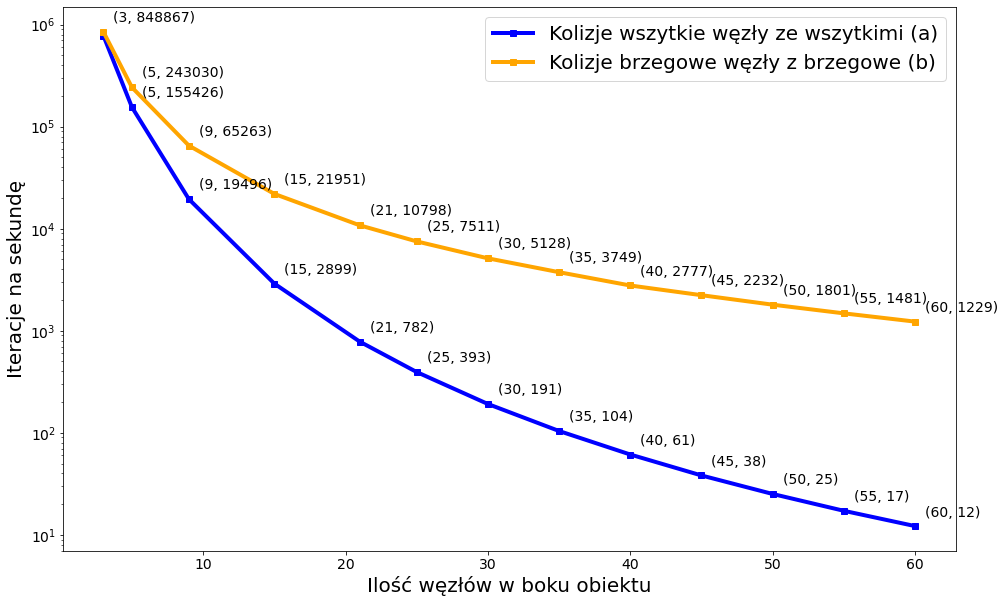
\includegraphics[width=15cm]{performance_side_size}
        \caption{
            Liczba iteracji na sekundę w zależności od 
            ilości węzłów w bokach obiektów dla dwóch metod obsługi zderzeń
        }
    \end{figure}

    Wersja algorytmu biorąca pod uwagę jedynie węzły brzegowe danych obiektów podczas obliczania kolizji cechuje 
    się wyraźnie zwiększoną wydajnością.

    \begin{table}[H]
        \centering
        \begin{tabular}{||c c c c||} 
            \hline
            węzły w boku obiektu & $iteracje / [s]$ dla (a) & $iteracje / [s]$ dla (b) & krotność przyśpieszenia \\ [0.5ex] 
            \hline\hline
            3 & 777633 & 848867 & 1.09 \\ 
            \hline
            5 & 155426 & 243030 & 1.56 \\
            \hline
            9 & 19496 & 65263 & 3.34 \\
            \hline
            15 & 2899 & 21951 & 7.57 \\
            \hline
            21 & 782 & 10798 & 13.79 \\
            \hline
            25 & 393 & 7511 & 19.06 \\
            \hline
            30 & 191 & 5128 & 26.76 \\
            \hline
            35 & 104 & 3749 & 36.00 \\
            \hline
            40 & 61 & 2777 & 45.33 \\ 
            \hline
            45 & 38 & 2232 & 58.43 \\ 
            \hline
            50 & 25 & 1801 & 71.63 \\
            \hline
            55 & 17 & 1481 & 86.11 \\ 
            \hline
            60 & 12 & 1229 & 100.88 \\ [1ex] 
            \hline
        \end{tabular}
        \caption{ Porównanie wydajności przypadku niezoptymalizowanego (a) i zoptymalizowanego (b) }
    \end{table}
    Dla większych obiektów zyski z zastosowanej optymalizacji są bardzo duże. W przypadku dwóch obiektów
    $60 \times 60$ ilość iteracji dla algorytmu zoptymalizowanego jest ponad $100$ razy większa.
        
    \section{Test rozrywania obiektu}
    \subsection{Opis testu}
    Jeden obiekt zostaje umieszczony nieruchomo przy podłożu, drugi znajduje się nad nim. Siła grawitacji
    jest aktywna, z tego powodu wolno spadający obiekt zderza się z obiektem stacjonarnym.
    Jeżeli odległość między dwoma połączonymi węzłami zwiększy się powyżej $1.5$ odległości równowagi dla 
    tego połączenia ($d_x$), połączenie to zostaje zerwane, w ten sposób symulujemy rozrywanie obiektów pod dużym 
    obciążeniem. Do obsługi kolizji została użyta wersja algorytmu każdy węzeł z każdym węzłem, ponieważ
    działa on poprawnie dla przenikających się obiektów a przy relatywnie niewielkiej liczbie 
    węzłów ($4$ i $288$) wciąż zapewnia bardzo dobrą płynność działania animacji.

        
    \subsection{Parametry symulacji}
    Parametry ogólne:
    \begin{itemize}
        \item $g = 9.81 [\frac{m}{s^2}]$
        \item $dt = 10^{-5}[s]$
    \end{itemize}
    Odpychanie międzyobiektowe:
    \begin{itemize}
        \item $V_{0} = 20$
        \item $d_{0} = 0.07$
    \end{itemize}
    Parametry obiektu $12 \times 24$:
    \begin{itemize}
        \item $c_{1} = 5.0$
        \item $m_{1} = 1.0$
        \item $d_{1} = 0.08$
        \item $V_{1} = 70.0$
        \item $p_{1} = [-0.92, -0.925]$
    \end{itemize}
    Parametry obiektu $2 \times 2$:
    \begin{itemize}
        \item $c_{2} = 1.0$
        \item $m_{2} = 30.0, 50.0, 80.0$
        \item $d_{2} = 0.15$
        \item $V_{2} = 500.0$
        \item $p_{2} = [-0.12, 0.8]$
    \end{itemize}
    Parametry $p_x$ oznaczają pozycję początkową obiektu, $m_x$ masę węzłow w obiekcie, 
    $d_x$ pozycję równowagi przyciągania/odpychania pomiędzy dwoma węzłami dla tego
    samego obiektu lub jedynie odpychania dla odziaływań międzywęzłowych,
    $V_x$ współczynnik odziaływania międzywęzłowego, $g$ przyśpieszenie grawitacyjne, 
    $c_x$ współcznnik oporu powietrza dla węzłów w obiekcie.

    \newpage
    \subsection{Wyniki dla 120 kg}
    \begin{figure}[h]

        \begin{subfigure}{0.5\textwidth}
            \centering
            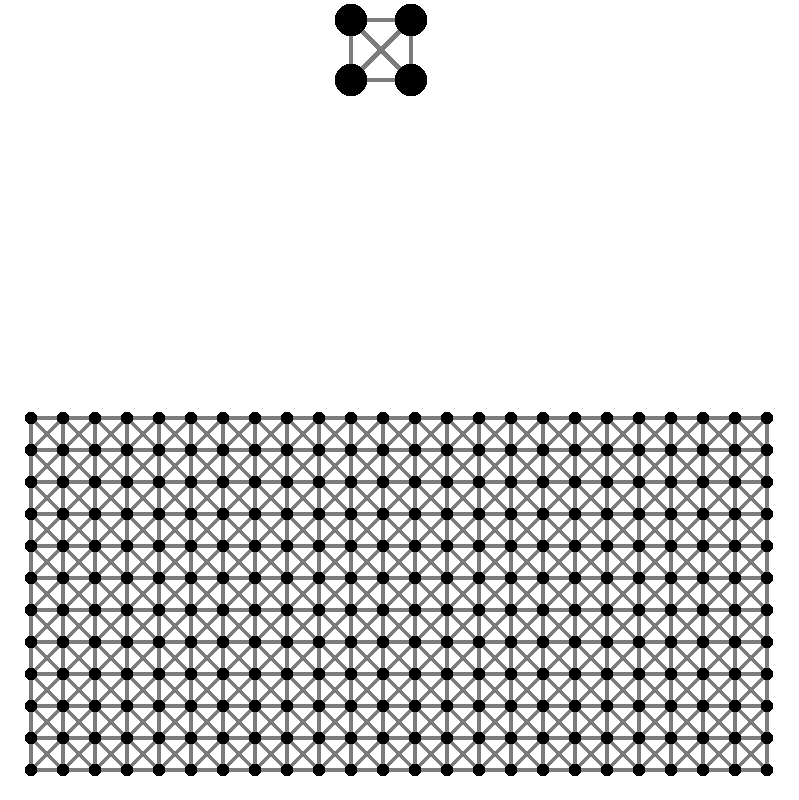
\includegraphics[width=6cm, height=6cm]{collision_2x2_24x12_mass30_1} 
            \caption{Stan początkowy}
        \end{subfigure}
        \begin{subfigure}{0.5\textwidth}
            \centering
            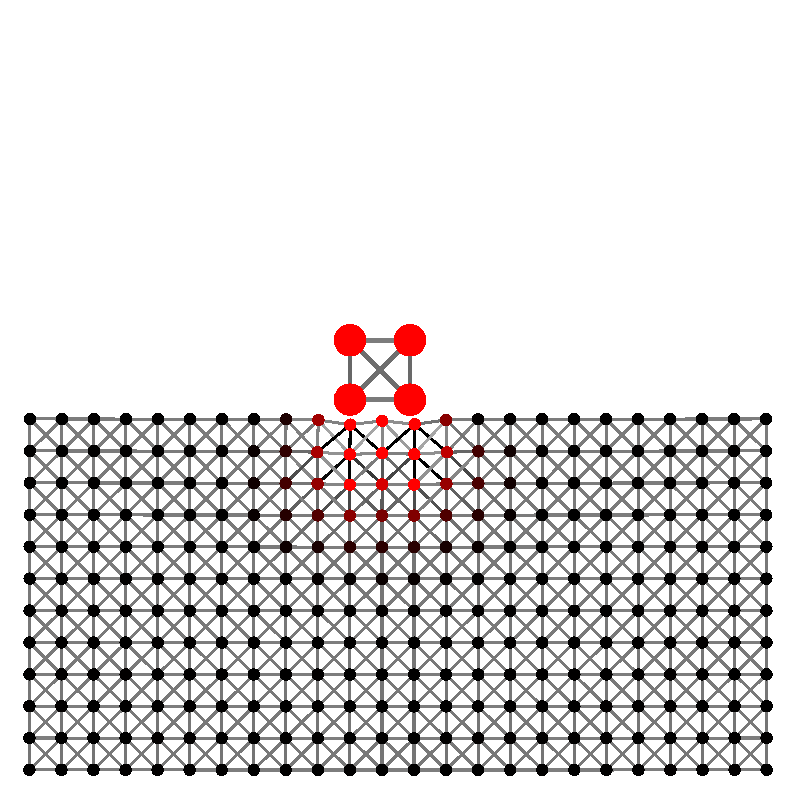
\includegraphics[width=6cm, height=6cm]{collision_2x2_24x12_mass30_2}
            \caption{Zderzenie}
        \end{subfigure}
        \begin{subfigure}{0.5\textwidth}
            \centering
            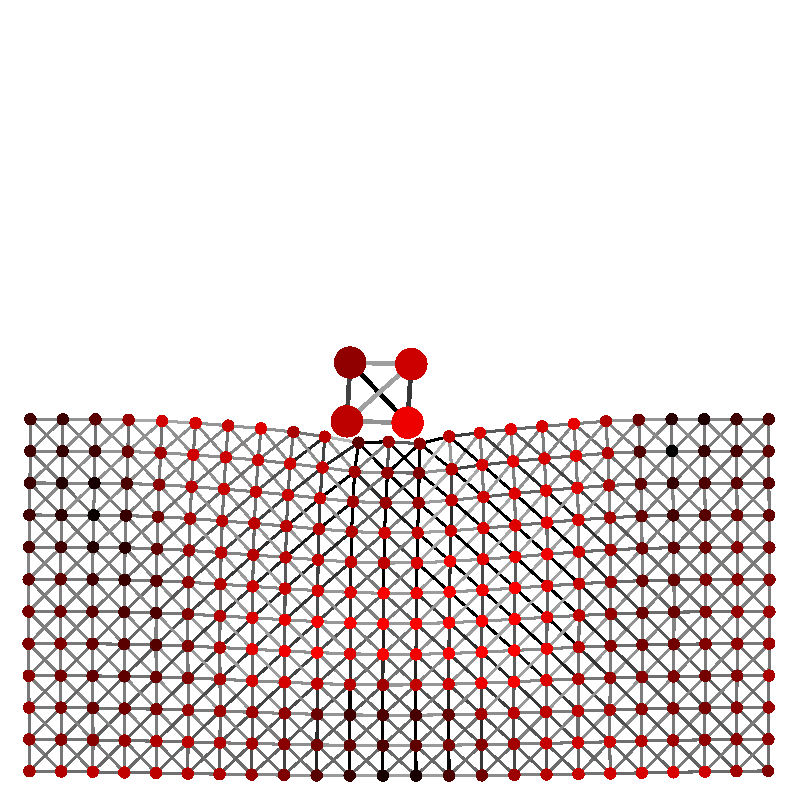
\includegraphics[width=6cm, height=6cm]{collision_2x2_24x12_mass30_3}
            \caption{Chwila po zderzeniu}
        \end{subfigure}
        \begin{subfigure}{0.5\textwidth}
            \centering
            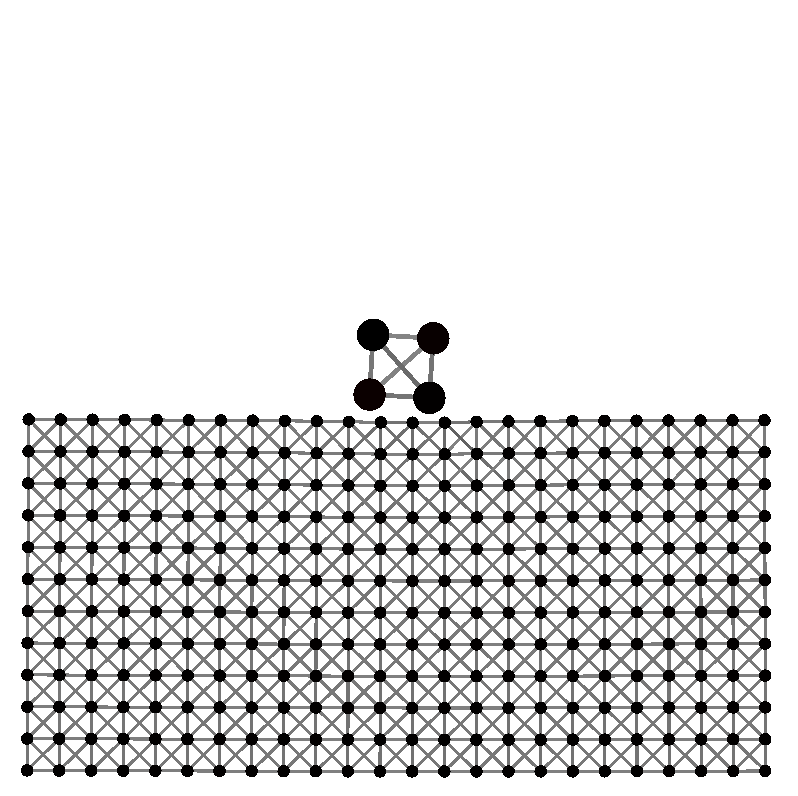
\includegraphics[width=6cm, height=6cm]{collision_2x2_24x12_mass30_4}
            \caption{Stan stabilny}
        \end{subfigure}
        
        \caption{Zderzenie spadającego obiektu $2 \times 2$ o masie 120 kg na obiekt $12 \times 24$ o masie 288 kg}
    \end{figure}
    Masa pojednczczego węzła w wolno spadającym obiekcie wynosi 30 kg co daje łączną masę równą 120 kg.
    Węzły o kolorze czarnym mają zerową energię kinetyczną, 
    zmienieją kolor na czerwony proporcjonalnie do ilości posiadanej energii kinetczynej. 
    Przy zderzeniu widoczny jest transfer energii kinetcznej z obiektu $2 \times 2$ do obiektu $12 \times 24$, 
    w którym po chwili zaczyna rozchodzić się fala. Ze względu na zastosowanie siły oporu proporcjonalnej do prękości
    po kilku sekundach układ stabilizuje się, obiekt $2 \times 2$ leży nieruchomo na obiekcie $12 \times 24$. 
    Żadne z połączeń międzywęzłowych nie zostało przerwane ze względu na zbyt niską energię zderzenia.

    \newpage
    \subsection{Wyniki dla 200 kg}
    \begin{figure}[h]

        \begin{subfigure}{0.5\textwidth}
            \centering
            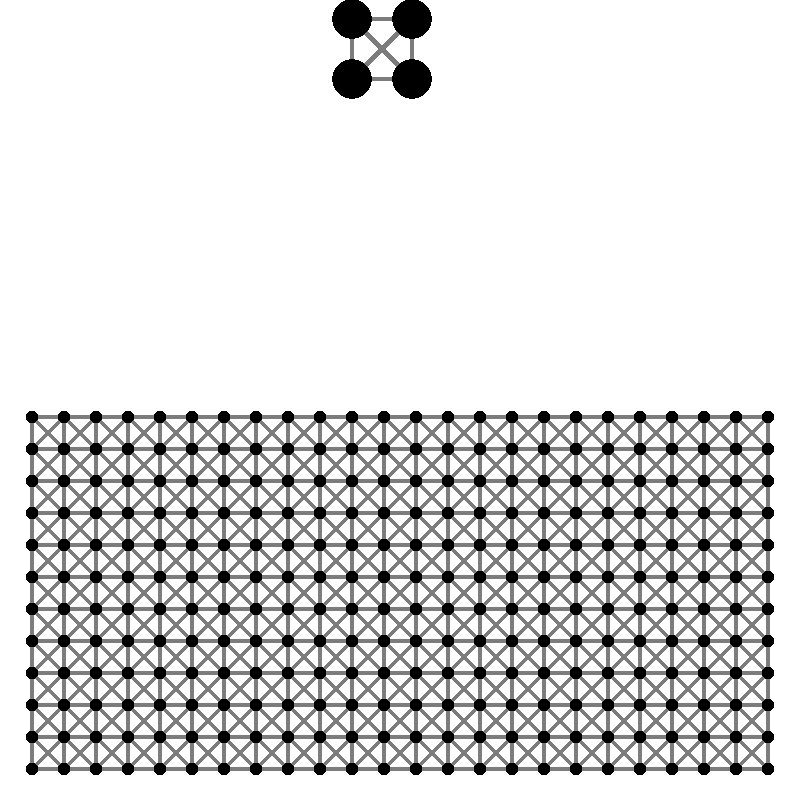
\includegraphics[width=6cm, height=6cm]{collision_2x2_24x12_mass50_1} 
            \caption{Stan początkowy}
        \end{subfigure}
        \begin{subfigure}{0.5\textwidth}
            \centering
            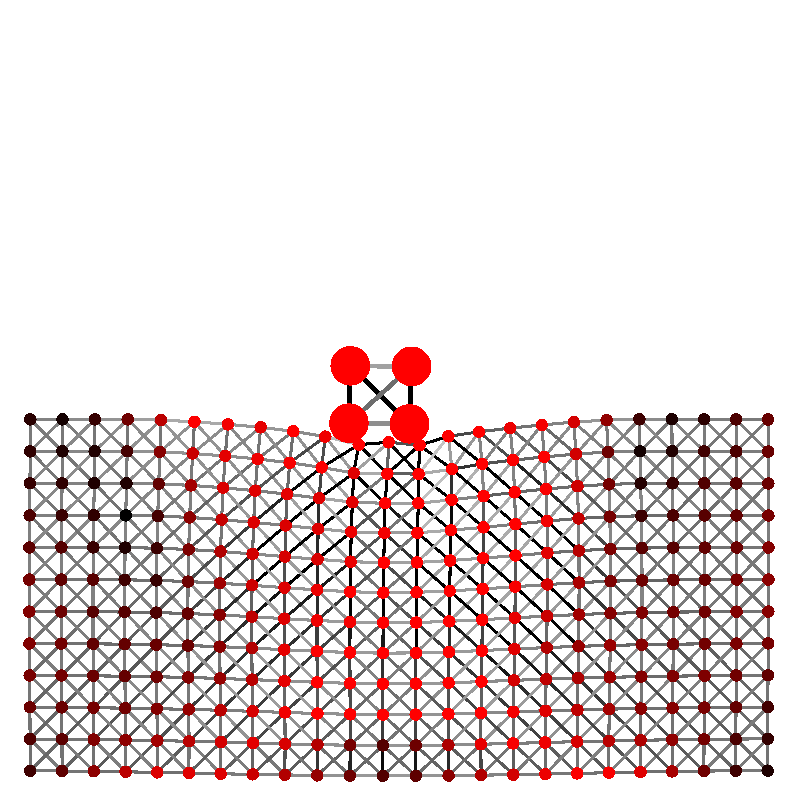
\includegraphics[width=6cm, height=6cm]{collision_2x2_24x12_mass50_2}
            \caption{Zderzenie}
        \end{subfigure}
        \begin{subfigure}{0.5\textwidth}
            \centering
            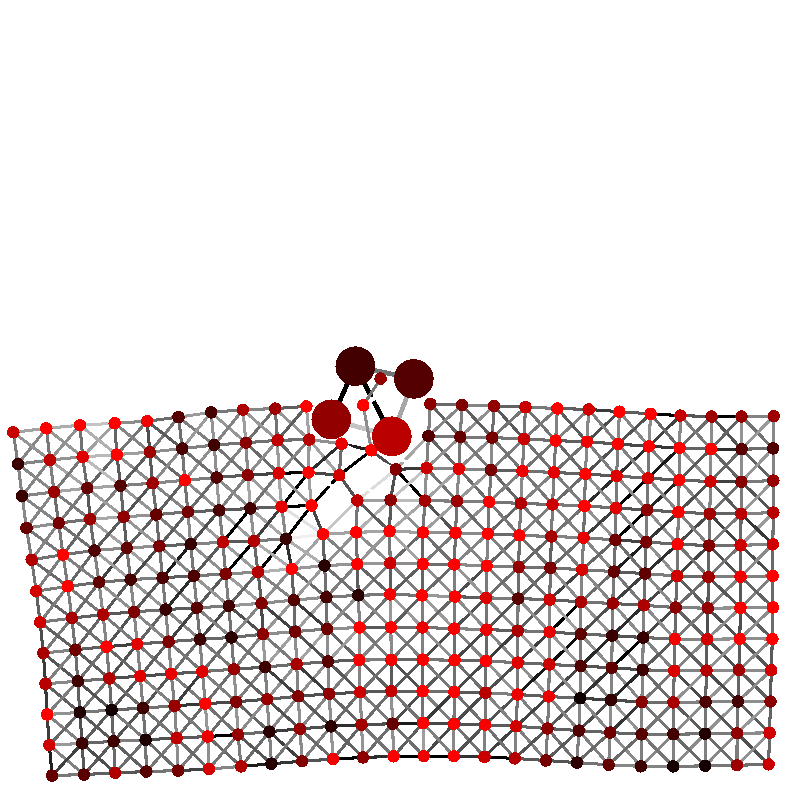
\includegraphics[width=6cm, height=6cm]{collision_2x2_24x12_mass50_3}
            \caption{Chwila po zderzeniu}
        \end{subfigure}
        \begin{subfigure}{0.5\textwidth}
            \centering
            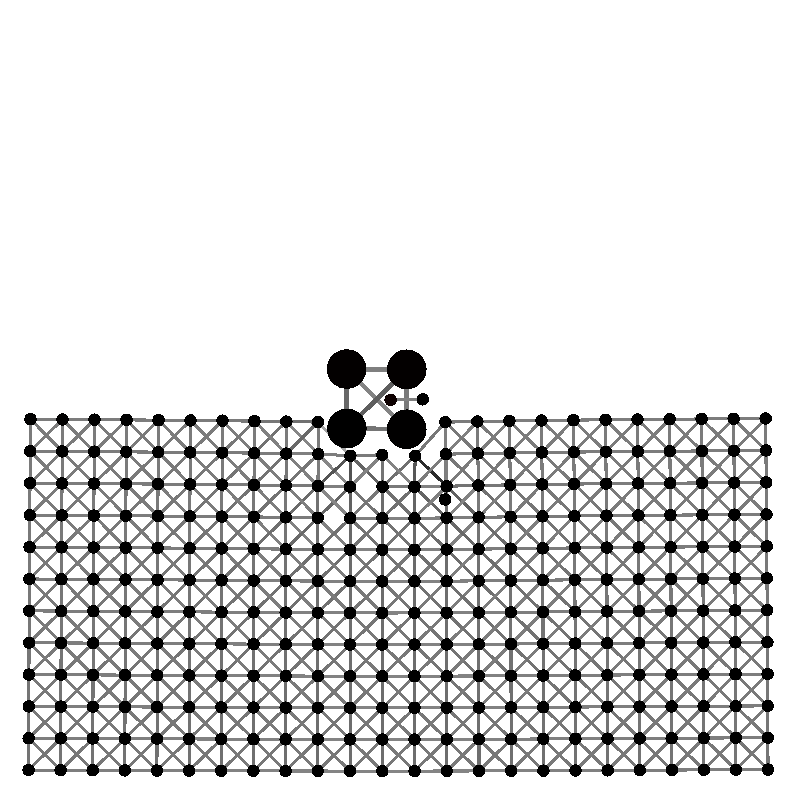
\includegraphics[width=6cm, height=6cm]{collision_2x2_24x12_mass50_4}
            \caption{Stan stabilny}
        \end{subfigure}
        
        \caption{Zderzenie spadającego obiektu $2 \times 2$ o masie 200 kg na obiekt $12 \times 24$ o masie 288 kg}
    \end{figure}

    Zwiększamy masę węzłów w obiekcie $2 \times 2$ z 30 kg do 50 kg. Ponieważ w reprezentacja wizualnej węzła jego pole 
    jest proporjonalne do jego masy, tym razem obiekt $2 \times 2$ jest większy.
    Większa energia kinetyczna przy zderzeniu powoduje przerwanie kilku połączeń międzywęzłowych, a obiekt $2 \times 2$ 
    utyka w wytworzonej dziurze. Część pierwotnego obiektu $12 \times 24$ oderwała się i utkneła w obiekcie $2 \times 2$.

    \newpage
    \subsection{Wyniki dla 320 kg}
    \begin{figure}[h]

        \begin{subfigure}{0.5\textwidth}
            \centering
            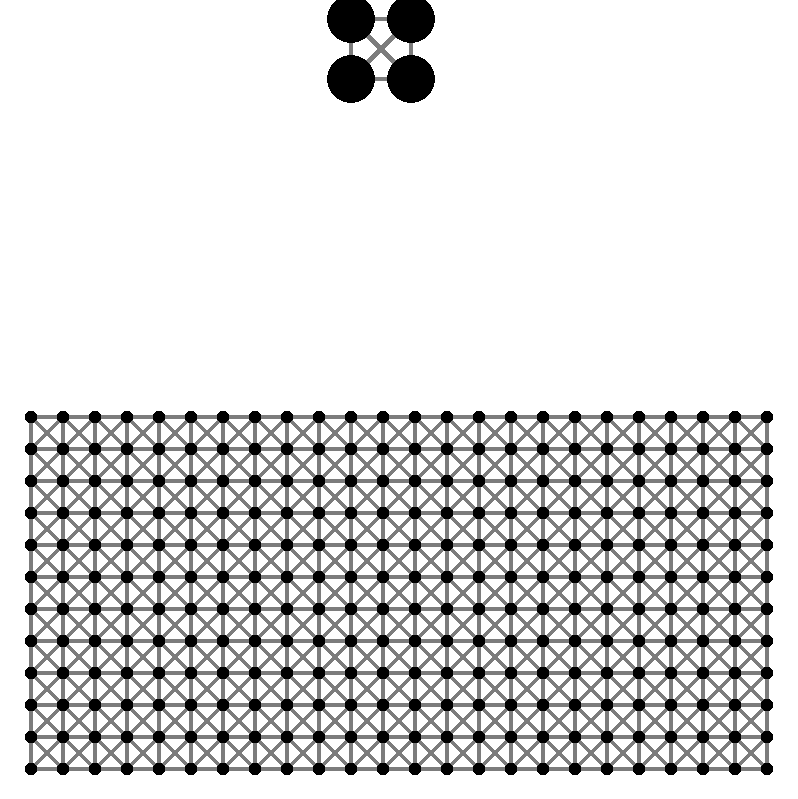
\includegraphics[width=6cm, height=6cm]{collision_2x2_24x12_mass80_1} 
            \caption{Stan początkowy}
        \end{subfigure}
        \begin{subfigure}{0.5\textwidth}
            \centering
            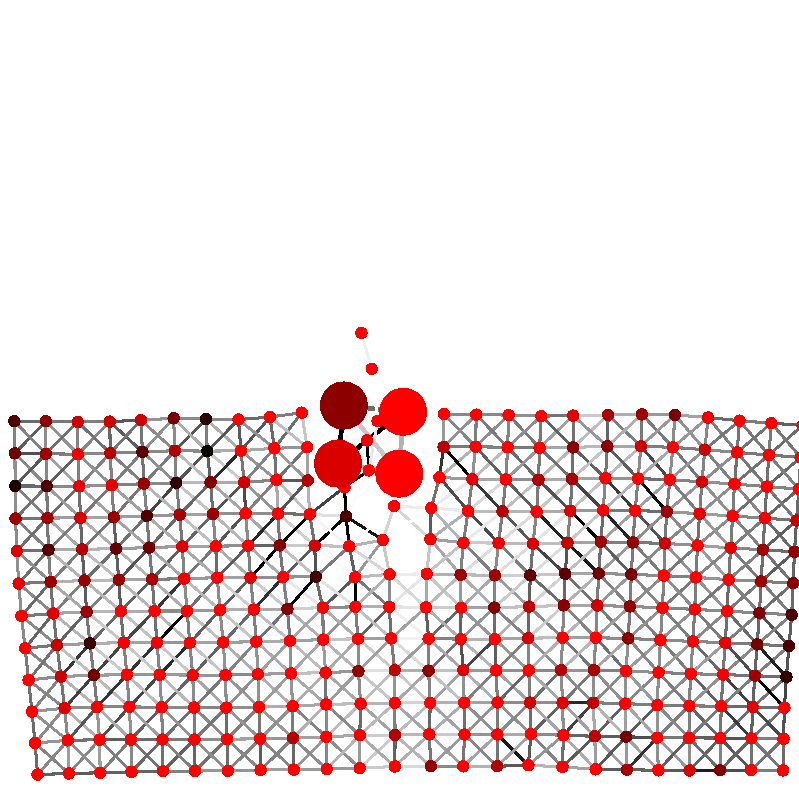
\includegraphics[width=6cm, height=6cm]{collision_2x2_24x12_mass80_2}
            \caption{Zderzenie}
        \end{subfigure}
        \begin{subfigure}{0.5\textwidth}
            \centering
            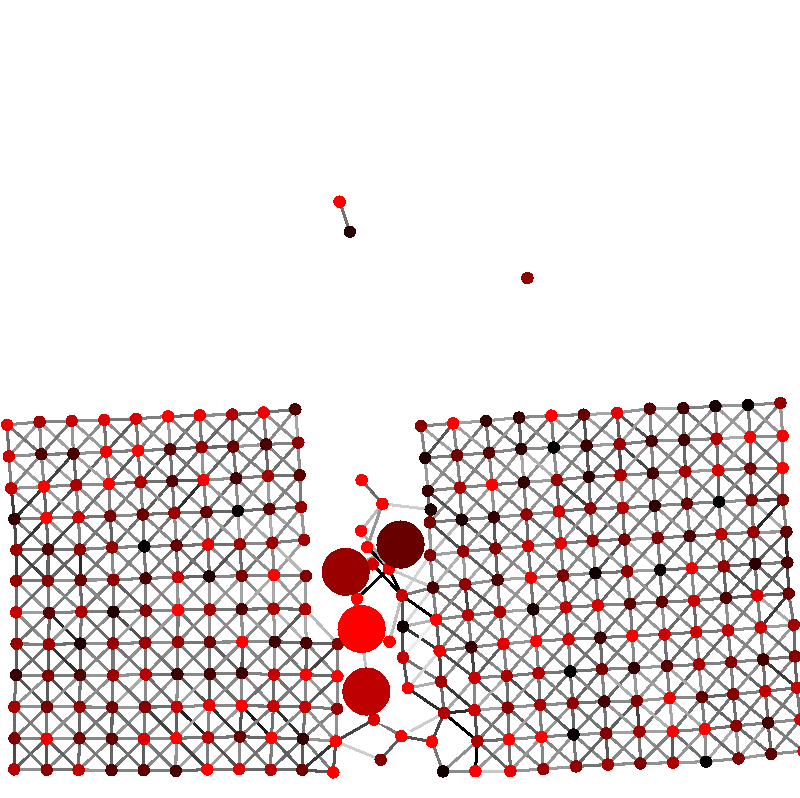
\includegraphics[width=6cm, height=6cm]{collision_2x2_24x12_mass80_3}
            \caption{Chwila po zderzeniu}
        \end{subfigure}
        \begin{subfigure}{0.5\textwidth}
            \centering
            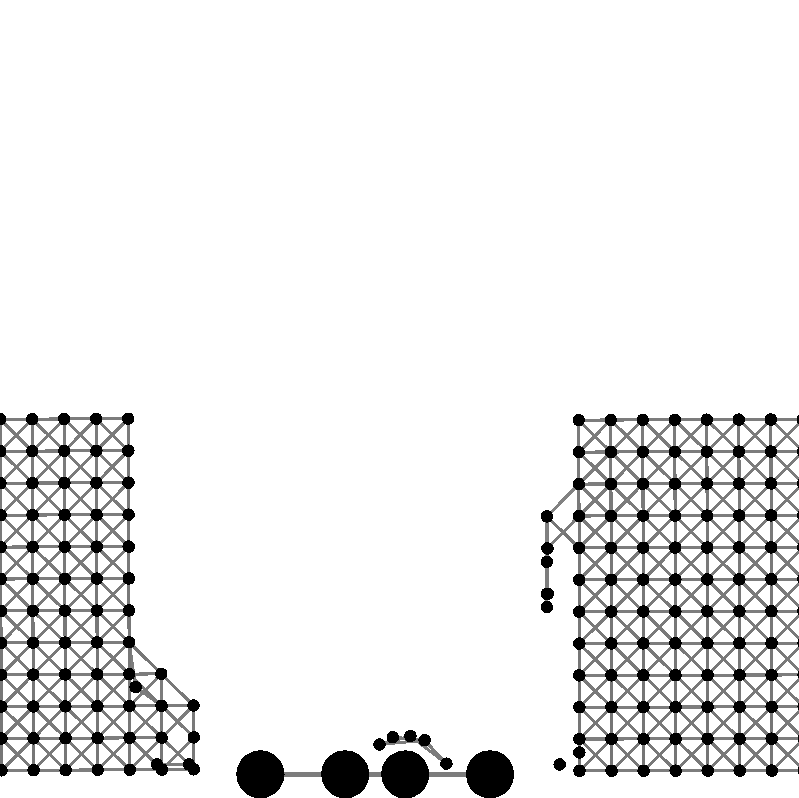
\includegraphics[width=6cm, height=6cm]{collision_2x2_24x12_mass80_4}
            \caption{Stan stabilny}
        \end{subfigure}
        
        \caption{Zderzenie spadającego obiektu $2 \times 2$ o masie 320 kg na obiekt $12 \times 24$ o masie 288 kg}
    \end{figure}

    Ponowne zwiększona została masa węzłów obiektu $2 \times 2$, tym razem z 50 kg do 80 kg, dając łączną masę 320 kg.
    W chwili zderzenia po obiekcie $12 \times 24$ rozchodzi się gwałtownie fala energii kinetycznej a on sam zostaje 
    rozerwany. Częściowemu zniszczeniu ulega również obiekt $2 \times 2$, ze względu duży stosunek masy do wytrzymałości
    połączeń międzywęzłowych niektóre z tych połączeń zostały przerwane.

\chapter{Podsumowanie}
    \section{Wnioski}
    Zastosowanie metoda dynamiki molekularnej daje bardzo interesujące 
    wyniki podczas symulacji zderzeń obiektów.

    \section{Dodatek}

    \subsection{Filmik prezentujące działanie aplikacji}

    \subsubsection{Przekazanie energii między dwoma sztywnimi obiektami}

    Mniejszy obiekt $3 \times 3$ po odbiciu od większego obiektu $8 \times  8$ znajdującego się 
    pod nim wznosi się na
    wysokość o wiele większą, niż ta z której rozpoczął spadek swobodny.
    Występuje tutaj przekazanie części energii z obiektu większego do mniejszego - sama zasada energii jest zachowana.
    \\
    \\
    \url{https://youtu.be/nolLh6CSa-8}

    \subsubsection{Przekazanie energii między dwoma miękkimi obiektami}
    W tym przypadku obiekty są mniej sztywne,
    obiekt $3 \times 3$ po odbiciu od obiektu $8 \times  8$ wznosi się na wyraźnie mniejszą wysokość niż w przypadku bardziej sztywnych obiektów
    (jednak wciąż wyżej niż punkt z którego zaczął spadać). Można to wytłumaczyć tym,
    że znaczna część energii która w poprzednim przypadku była częścią ruchu postępowego,
    teraz stała się energią wewnętrzną obiektów (wibracje obiektów pochłaniają część energii).
    \\
    \\
    \url{https://youtu.be/q2uYx8uLl3w}

    \subsubsection{Proste zderzenie dwóch obiektów}
    \url{https://www.youtube.com/watch?v=4cGcL_5yUt4}

    \subsubsection{Zderzenie obiektów 120 kg z 288 kg}
    \url{https://youtu.be/3dV6EpRacyA}

    \subsubsection{Zderzenie obiektów 200 kg z 288 kg}
    \url{https://youtu.be/lRGl7CJiqFU}

    \subsubsection{Zderzenie obiektów 320 kg z 288 kg}
    \url{https://youtu.be/VYeCsaqNxAY}

    \subsection{Repozytorium}
    \subsubsection{Link do repozytorium z kodem}
    \url{https://github.com/theYiome/elastic-objects-rs}

\end{document}